\section{Lösungsidee}
	\begin{wrapfigure}{r}{0.35\textwidth}
		\setlength\intextsep{0pt}
		\centering
		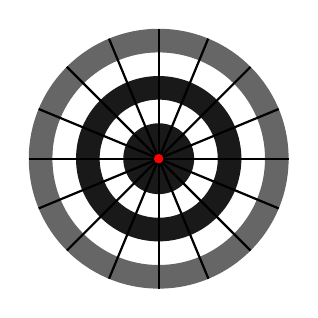
\begin{tikzpicture}[scale=0.3]
	\fill[black!90!white] (0,0) circle [radius=1.5];
	\fill[black!90!white, even odd rule] (0,0) circle[radius=2.5] circle[radius=3.5];
	\fill[black!60!white, even odd rule] (0,0) circle[radius=4.5] circle[radius=5.5];

	\foreach \angle in {0, 22.5, 45, 67.590, 90, 112.5, 135, 157.5, 180, 202.5, 225, 247.5, 270, 292.5, 315, 337.5} 
    	\draw[thick] (0,0) -- (\angle:5.5);

	\fill[red] (0,0) circle[radius=0.2];
\end{tikzpicture}

		\caption{Geraden}
		\label{abb:spidergrafik}
		\vspace{-20pt}
	\end{wrapfigure}
	Zunächst habe ich den \task{} mit TikZ nachgezeichnet, um den genauen Aufbau durch Nachbau zu verstehen. Die 16 gleichgroßen Kreissegmente sind durch Strahlen getrennt, die im Abstand von \(22,5^{\circ}\) vom Pol (dem Mittelpunkt) aus gezeichnet werden. Der Abstand zwischen den Strahlen beträgt im Bogenmaß \(\frac{22,5\pi}{180}\).

	Für die Dekodierung steht mir aus dem Kreismittelpunkterkennungsprozess die Liste der Kreismittelpunkte zur Verfügung. Die Kreisdurchmesser entsprechen der Länge der Zusammenhangskomponenten an den Mittelpunktskoordinaten. Mit diesen Informationen kann ich dank bekannter Proportionen eines \task{}s auf die Position des äußeren Ringes, der die Informationen trägt, schließen (siehe Abb. \ref{abb:dims}). Wie in der Lösungsidee zur Kreismittelpunkterkennung festgestellt gilt \(u=\frac{1}{3}d\).

	\begin{wrapfigure}{r}{0.25\textwidth}
		\setlength\intextsep{0pt}
		\centering	
		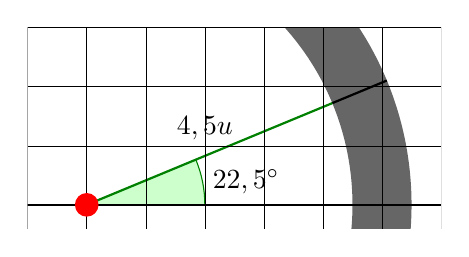
\begin{tikzpicture}[scale=0.75]
	\clip (-1,-0.4) rectangle (6, 3);
	\fill[black!60!white, even odd rule] (0,0) circle[radius=4.5] circle[radius=5.5];

	\foreach \angle in {0, 22.5, 45, 67.590, 90, 112.5, 135, 157.5, 180, 202.5, 225, 247.5, 270, 292.5, 315, 337.5} 
    	\draw[thick] (\angle:4.5) -- (\angle:5.5);

	\filldraw[fill=green!20,draw=green!50!black] (0,0) -- (2,0) arc[start angle=0, end angle=22.5, radius=2];
	\draw[green!50!black, thick] (0,0) -- (22.5:4.5);

	\draw (2, 1.3) node {\(4,5u\)};
	\draw (2.7, 0.4) node {\(22,5^{\circ}\)};

	\draw[very thin] (-6, -6) grid (6, 6);
	\draw[thick] (-6, 0) -- (6, 0);
	\fill[red] (0,0) circle[radius=0.2];
\end{tikzpicture}
		\caption{}
		\label{abb:trigon}
	\end{wrapfigure}
	Daher kann ich mithilfe von polaren Koordinaten\footnote{\url{https://www.lernhelfer.de/schuelerlexikon/mathematik-abitur/artikel/polarkoordinatensystem}} die Strecken, die die Kreisringe in Segmente einteilen, bestimmen. Jede der Strecken ist Teil eines Strahls, der am Mittelpunkt in einem Vielfachen von \(22,5^{\circ}\) beginnt. Die eigentlichen Strecken, die auf dem äußeren Kreisring liegen, beginnen nach einem Abstand von \(4,5u\) und enden bei \(5,5u\). Die Anfangs- und Endpunkte aller Strecken lauten also:

	\begin{displaymath}
	A(k \cdot 22,5^{\circ}:4,5u) \hspace{2em} B(k \cdot 22,5^{\circ}:5,5u) \hspace{2em} k = \{\mathbb{N}_0 \hspace{0.3em}|\hspace{0.3em} 0 \le x \le 15\}
	\end{displaymath}

	Da der Strahl zusammen mit der Achse, von der aus der Winkel gemessen wird, ein rechtwinkliges Dreieck bildet (s. Abb \ref{abb:trigon}), könnenen wir die Punkte der Strecke in kartesischen Koordinaten berechnen. Ich habe das Koordinatensystem in der Einheit \(u\) gezeichnet. Bitte stellen sie Ihren Taschenrechner vorher auf "`rad"' ein!

	\begin{gather}
	k = \{\mathbb{N}_0 \hspace{0.3em}|\hspace{0.3em} 0 \le x \le 15\} \\
	\begin{split}
	x_{innen} &= cos(k \cdot \frac{22,5\pi}{180}) \cdot 4,5u \\
	y_{innen} &= sin(k \cdot \frac{22,5\pi}{180}) \cdot 4,5u
	\end{split}
	\hspace{5em}
	\begin{split}
	x_{aussen} &= cos(k \cdot \frac{22,5\pi}{180}) \cdot 5,5u \\
	y_{aussen} &= sin(k \cdot \frac{22,5\pi}{180}) \cdot 5,5u
	\end{split}
	\end{gather}

	\begin{figure}[!ht]
		\begin{subfigure}[b]{0.5\textwidth}
			\centering	
			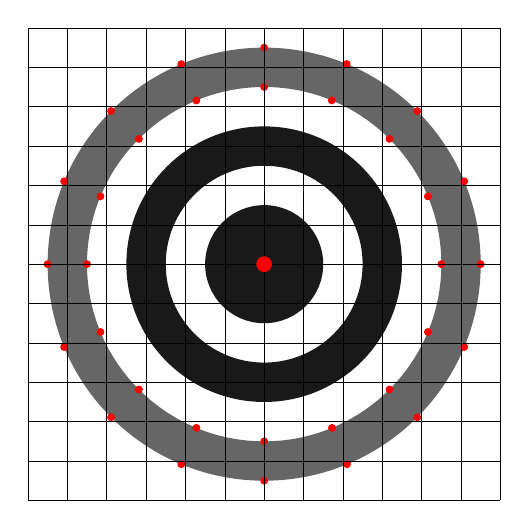
\begin{tikzpicture}[scale=0.5]
	\fill[black!90!white] (0,0) circle [radius=1.5];
	\fill[black!90!white, even odd rule] (0,0) circle[radius=2.5] circle[radius=3.5];
	\fill[black!60!white, even odd rule] (0,0) circle[radius=4.5] circle[radius=5.5];
	
	\foreach \angle in {0, 22.5, 45, 67.590, 90, 112.5, 135, 157.5, 180, 202.5, 225, 247.5, 270, 292.5, 315, 337.5} 
    		\fill[red] (\angle:4.5) circle [radius=0.1] (\angle:5.5) circle [radius=0.1]; 

	\draw[very thin] (-6, -6) grid (6, 6);
	\fill[red] (0,0) circle[radius=0.2];
\end{tikzpicture}
			\caption{Einteilende Punkte}
		\end{subfigure}
		\begin{subfigure}[b]{0.5\textwidth}
			\centering	
			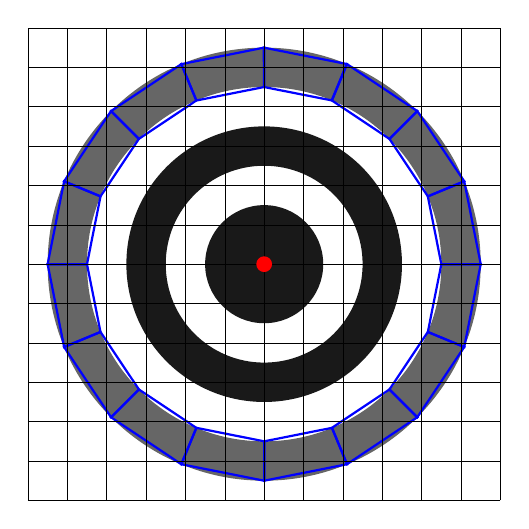
\begin{tikzpicture}[scale=0.5]
	\fill[black!90!white] (0,0) circle [radius=1.5];
	\fill[black!90!white, even odd rule] (0,0) circle[radius=2.5] circle[radius=3.5];
	\fill[black!60!white, even odd rule] (0,0) circle[radius=4.5] circle[radius=5.5];

	\foreach \angle in {0, 22.5, 45, 67.590, 90, 112.5, 135, 157.5, 180, 202.5, 225, 247.5, 270, 292.5, 315, 337.5} 
    	\draw[blue, thick] (\angle:4.5) -- (\angle:5.5) -- (\angle+22.5:5.5) -- (\angle+22.5:4.5) -- cycle;

    	
	\draw[very thin] (-6, -6) grid (6, 6);
	\fill[red] (0,0) circle[radius=0.2];
\end{tikzpicture}
			\caption{Trapeze}
		\end{subfigure}
	\end{figure}

	Wenn wir nun alle benachbarten Koordinaten verbinden, erhalten wir 16 Trapeze, die fast den Kreissegmenten entsprechen. Da die Abweichung zwischen dem jeweiligen Trapez und dem jeweiligen Kreissegment sehr gering ist, kann aus den Pixeln im Trapez auf die Farbe des Ringsegmentes geschlossen werden. Da das ganze Ringsegment entweder ganz weiß oder ganz schwarz ist, entspricht die vorherrschende Farbe im Trapez der Farbe des Kreissegmentes.
\section{Umsetzung}
	Die vorherrschende Farbe kann mit einer Flood-Fill über die Trapezfläche ausgezählt werden. Hierfür benötigen wir zum einen für jedes der 16 Trapeze einen Startpunkt. Zum anderen muss für die Flood-Fill die Linien des Trapezes bestimmt werden, sodass die Flut die Trapezfläche nicht verlässt.

	Für die Bestimmung der Startpunkte nummerieren ich die Segmente von 0 bis 15. Wenn man nun die x- und y-Koordinaten aller anliegende Punkte arithmetisch mittelt, erhält man den Mittelpunkt des Trapezes. Die Formel für die Koordinaten eines \textit{n}ten-Trapezes eines Kreis-Codes mit dem Mittelpunkt \(x_0 . y_0\) lautet:
	\begin{gather}
	\begin{split}
		x_1 &= cos(n \cdot \frac{22,5\pi}{180}) \cdot 5,5u + x_0\\
		y_1 &= sin(n \cdot \frac{22,5\pi}{180}) \cdot 5,5u + y_0\\ \vspace{2em}
		x_2 &= cos(n \cdot \frac{22,5\pi}{180}) \cdot 4,5u + x_0\\
		y_2 &= sin(n \cdot \frac{22,5\pi}{180}) \cdot 4,5u + y_0
	\end{split}
	\hspace{5em}
	\begin{split}
		x_3 &= cos((n+1) \cdot \frac{22,5\pi}{180}) \cdot 5,5u + x_0\\
		y_3 &= sin((n+1) \cdot \frac{22,5\pi}{180}) \cdot 5,5u + y_0 \\ \vspace{2em}
		x_4 &= cos((n+1) \cdot \frac{22,5\pi}{180}) \cdot 4,5u + x_0\\
		y_4 &= sin((n+1) \cdot \frac{22,5\pi}{180}) \cdot 4,5u + y_0
	\end{split} \label{eq:nKoords}
	\end{gather}
	\begin{equation}
	x = \frac{(x_1+x_2+x_3+x_4)}{4} \hspace{4em} y = \frac{(y_1+y_2+y_3+y_4)}{4}
	\end{equation}
	Abschließend müssen die x- und y-Werte noch gerundet werden, da im gerasterten Bild nur ganzzahlige Pixel adressierbar sind.
	Zur Überprüfung habe ich ein kleines CPP-Programm geschrieben, welches die Formel für \(n = 0\hspace{2pt}..\hspace{2pt}15 \) durchrechnet und entstprechende TikZ-Anweisungen ausgibt (Quellcode: mittelpunkte.cpp). Obwohl sehr ungenau auf Vielfache von \(u\) gerundet wurde, liegen alle Punkte in ihrem jeweiligen Segment.
	\begin{figure}[!ht]
		\centering
		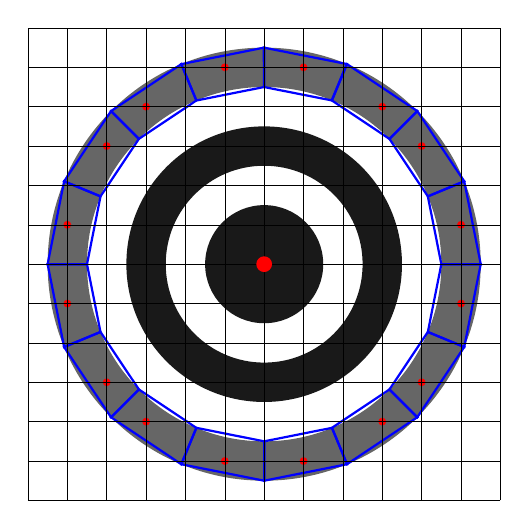
\begin{tikzpicture}[scale=0.5]
	\fill[black!90!white] (0,0) circle [radius=1.5];
	\fill[black!90!white, even odd rule] (0,0) circle[radius=2.5] circle[radius=3.5];
	\fill[black!60!white, even odd rule] (0,0) circle[radius=4.5] circle[radius=5.5];
	
	\fill[red] (5,1) circle [radius=0.1]; 
	\fill[red] (4,3) circle [radius=0.1]; 
	\fill[red] (3,4) circle [radius=0.1]; 
	\fill[red] (1,5) circle [radius=0.1]; 
	\fill[red] (-1,5) circle [radius=0.1]; 
	\fill[red] (-3,4) circle [radius=0.1]; 
	\fill[red] (-4,3) circle [radius=0.1]; 
	\fill[red] (-5,1) circle [radius=0.1]; 
	\fill[red] (-5,-1) circle [radius=0.1]; 
	\fill[red] (-4,-3) circle [radius=0.1]; 
	\fill[red] (-3,-4) circle [radius=0.1]; 
	\fill[red] (-1,-5) circle [radius=0.1]; 
	\fill[red] (1,-5) circle [radius=0.1]; 
	\fill[red] (3,-4) circle [radius=0.1]; 
	\fill[red] (4,-3) circle [radius=0.1]; 
	\fill[red] (5,-1) circle [radius=0.1];  

	\foreach \angle in {0, 22.5, 45, 67.590, 90, 112.5, 135, 157.5, 180, 202.5, 225, 247.5, 270, 292.5, 315, 337.5} 
	\draw[blue, thick] (\angle:4.5) -- (\angle:5.5) -- (\angle+22.5:5.5) -- (\angle+22.5:4.5) -- cycle;

	\draw[very thin] (-6, -6) grid (6, 6);
	\fill[red] (0,0) circle[radius=0.2];
\end{tikzpicture}
		\caption{Mittelpunkte}
	\end{figure}

	Um die Flood-Fill durchführen zu können, müssen nun die Grenzen der Trapeze bestimmt werden. 

	Alle Trapeze im Kreisring bestehen aus 16 Strecken, die den Kreisring einteilen sowie 16 obere- wie untere Strecken. Daher muss ich in die Grafiken für jedes \textit{n} folgende Punkte aus Gleichung \eqref{eq:nKoords} verbinden.:
	
	\begin{equation}
		\overline{P_1P_2} \hspace{3em}
		\overline{P_2P_4} \hspace{3em}
		\overline{P_1P_3} \hspace{3em}
	\end{equation}

	Wenn ich diese Strecken nun in eine weiteres Array einzeichne, erhalte ich Grenzen für die Flut von den soeben berechneten Mittelpunkten aus. Arrays entsprechen einer Rastergrafik. Das Einzeichen von geometrischen Formen in Rastergrafiken wird in der Literatur \texit{rastern} genannt. Meine Anforderungen an den Rasterisierungsalgorithmus lauten:
	\begin{itemize}
		\item Möglichst geringe Laufzeit
		\item Lückenlosigkeit, d.h die Linie muss ein durchgehender Pfad durch die Rastergrafik sein
	\end{itemize}
	Ausdrücklich nicht benötigt wird eine besonders schöne oder besonders genaue Rasterisierung, es muss nur ein möglichst großer Teil des Trapezes innerhalb der Linien liegen. Die gerasterten Linien werden dem Nutzer außerhalb von Debug-Funktionen niemals angezeigt.

	Ich habe mich über Rasteralgorithmen in einer Zusammenfassung eines Proseminars an der TU Dresden\footnote{\url{https://www.inf.tu-dresden.de/content/institutes/smt/cg/teaching/seminars/ProseminarSS08/skurfuerst/latex-doc.pdf}} informiert. Das PDF habe ich der Einsendung beigefügt.
	
	Der auf den Seiten 3 bis 5 und in einem YouTube-Talk\footnote{\url{https://youtu.be/zytBpLlSHms}} vorgestellte Bresenham-Algorithmus trifft mein Anforderungsprofil genau: Er zeichnet in Linearzeit eine 1px breite Linie zwischen zwei Punkten. Da der Algorithmus ausschließlich mit Ganzzahlen arbeitet, müssen alle Koordinaten vor Eingabe in den Algorithmus gerundet werden.
\section{Beispiele}